\documentclass[border={20.000000bp 20.000000bp 20.000000bp 30.000000bp}, 11pt]{standalone}
\pdfinfoomitdate=1
\pdftrailerid{}
\pdfsuppressptexinfo=1
\pdfinfo{ /Creator () /Producer () }

\usepackage{tikz}
\usepackage{xcolor}
\usetikzlibrary{shapes.misc}
\usetikzlibrary{backgrounds}

\definecolor{dotColorA}{HTML}{1F77B4}
\definecolor{dotColorB}{HTML}{FF7F0E}
\definecolor{dotColorC}{HTML}{2CA02C}
\definecolor{dotColorD}{HTML}{D62728}
\definecolor{dotColorE}{HTML}{9467BD}
\definecolor{dotColorF}{HTML}{8C564B}
\definecolor{dotColorG}{HTML}{E377C2}
\definecolor{dotColorH}{HTML}{7F7F7F}
\definecolor{dotColorI}{HTML}{BCBD22}
\definecolor{dotColorJ}{HTML}{17BECF}

\definecolor{labelBgColorA}{HTML}{1F77B4}
\definecolor{labelBgColorB}{HTML}{FF7F0E}
\definecolor{labelBgColorC}{HTML}{2CA02C}
\definecolor{labelBgColorD}{HTML}{D62728}
\definecolor{labelBgColorE}{HTML}{9467BD}
\definecolor{labelBgColorF}{HTML}{8C564B}
\definecolor{labelBgColorG}{HTML}{E377C2}
\definecolor{labelBgColorH}{HTML}{7F7F7F}
\definecolor{labelBgColorI}{HTML}{BCBD22}
\definecolor{labelBgColorJ}{HTML}{17BECF}

\definecolor{labelTextColorA}{HTML}{FFFFFF}
\definecolor{labelTextColorB}{HTML}{FFFFFF}
\definecolor{labelTextColorC}{HTML}{FFFFFF}
\definecolor{labelTextColorD}{HTML}{FFFFFF}
\definecolor{labelTextColorE}{HTML}{FFFFFF}
\definecolor{labelTextColorF}{HTML}{FFFFFF}
\definecolor{labelTextColorG}{HTML}{FFFFFF}
\definecolor{labelTextColorH}{HTML}{FFFFFF}
\definecolor{labelTextColorI}{HTML}{FFFFFF}
\definecolor{labelTextColorJ}{HTML}{FFFFFF}

\definecolor{linkColorA}{HTML}{1F77B4}
\definecolor{linkColorB}{HTML}{FF7F0E}
\definecolor{linkColorC}{HTML}{2CA02C}
\definecolor{linkColorD}{HTML}{D62728}
\definecolor{linkColorE}{HTML}{9467BD}
\definecolor{linkColorF}{HTML}{8C564B}
\definecolor{linkColorG}{HTML}{E377C2}
\definecolor{linkColorH}{HTML}{7F7F7F}
\definecolor{linkColorI}{HTML}{BCBD22}
\definecolor{linkColorJ}{HTML}{17BECF}

\def\textA{Online class upto: 12, 4}
\def\textB{Thesis pre-defence: April 14}
\def\textC{Thesis final defence: May 20}
\def\textD{CIP application due}
\def\textE{CIP class start}
\def\textF{CIP class end}
\def\textG{EID}
\def\textH{today}
\def\textI{DM Lab viva}
\def\textJ{DM Lab 3}

\begin{document}
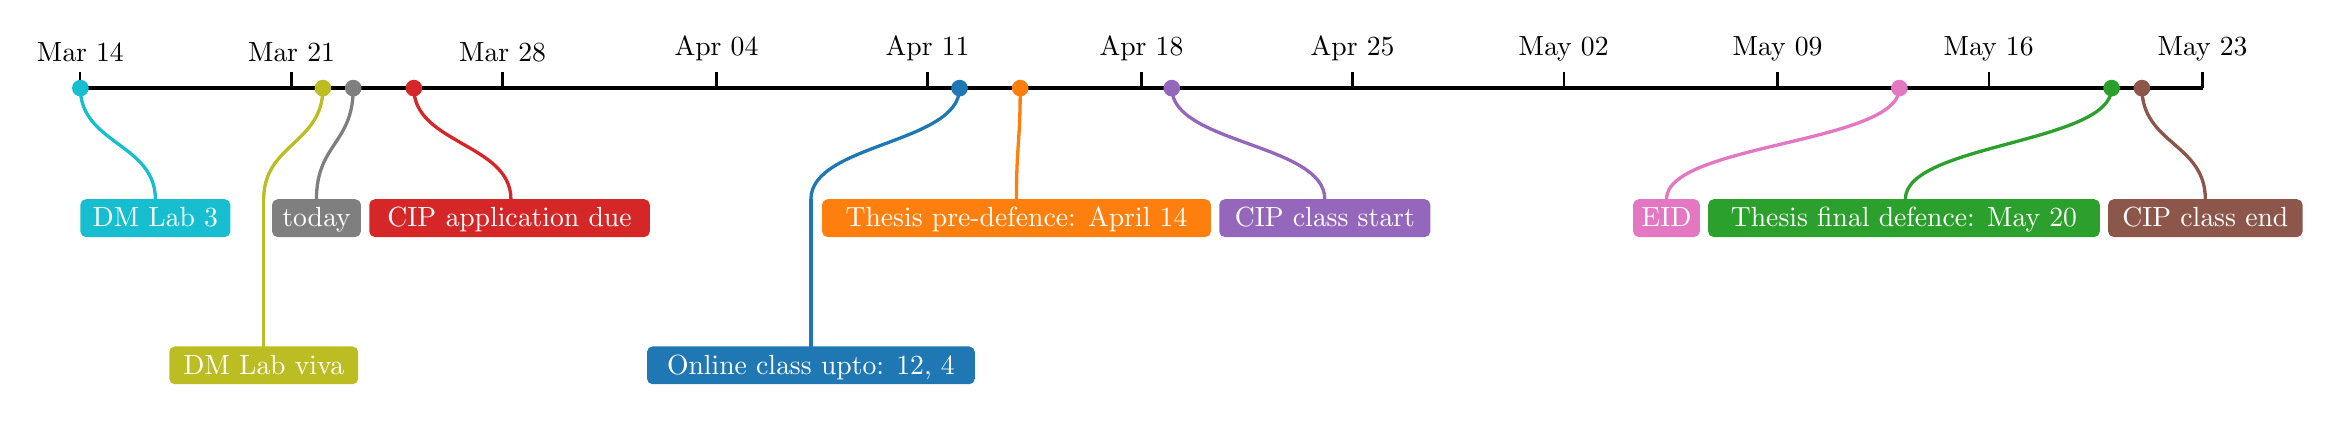
\begin{tikzpicture}[x=1bp,y=-1bp]

% shift for the margin
\begin{scope}[shift={(20, 20)}]
% main layer
\begin{scope}[shift={(0, 0)}]
% axis
\begin{scope}
\draw[very thick] (0, 0) -- (764, 0);
\end{scope}

% axis layer
\begin{scope}
\begin{scope}[shift={(0, 0)}]
\draw[thick] (0, -0) -- (0, 6pt)
node[anchor=south] {Mar 14};
\end{scope}
\begin{scope}[shift={(76, 0)}]
\draw[thick] (0, -0) -- (0, 6pt)
node[anchor=south] {Mar 21};
\end{scope}
\begin{scope}[shift={(152, 0)}]
\draw[thick] (0, -0) -- (0, 6pt)
node[anchor=south] {Mar 28};
\end{scope}
\begin{scope}[shift={(229, 0)}]
\draw[thick] (0, -0) -- (0, 6pt)
node[anchor=south] {Apr 04};
\end{scope}
\begin{scope}[shift={(305, 0)}]
\draw[thick] (0, -0) -- (0, 6pt)
node[anchor=south] {Apr 11};
\end{scope}
\begin{scope}[shift={(382, 0)}]
\draw[thick] (0, -0) -- (0, 6pt)
node[anchor=south] {Apr 18};
\end{scope}
\begin{scope}[shift={(458, 0)}]
\draw[thick] (0, -0) -- (0, 6pt)
node[anchor=south] {Apr 25};
\end{scope}
\begin{scope}[shift={(534, 0)}]
\draw[thick] (0, -0) -- (0, 6pt)
node[anchor=south] {May 02};
\end{scope}
\begin{scope}[shift={(611, 0)}]
\draw[thick] (0, -0) -- (0, 6pt)
node[anchor=south] {May 09};
\end{scope}
\begin{scope}[shift={(687, 0)}]
\draw[thick] (0, -0) -- (0, 6pt)
node[anchor=south] {May 16};
\end{scope}
\begin{scope}[shift={(764, 0)}]
\draw[thick] (0, -0) -- (0, 6pt)
node[anchor=south] {May 23};
\end{scope}
\end{scope}

% link layer
\begin{scope}
\draw[color=linkColorA, very thick] (316.51428571, 0.00000000) .. controls
(316.51428571, 20.00000000) and (263.00000000, 20.00000000) .. (263.00000000, 40.00000000);
\draw[color=linkColorA, very thick] (263.00000000, 40.00000000) -- (263.00000000, 53.60416000);
\draw[color=linkColorA, very thick] (263.00000000, 53.60416000) .. controls
(263.00000000, 73.60416000) and (263.00000000, 73.60416000) .. (263.00000000, 93.60416000);
\draw[color=linkColorB, very thick] (338.34285714, 0.00000000) .. controls
(338.34285714, 20.00000000) and (337.00000000, 20.00000000) .. (337.00000000, 40.00000000);
\draw[color=linkColorC, very thick] (731.25714286, 0.00000000) .. controls
(731.25714286, 20.00000000) and (657.00000000, 20.00000000) .. (657.00000000, 40.00000000);
\draw[color=linkColorD, very thick] (120.05714286, 0.00000000) .. controls
(120.05714286, 20.00000000) and (155.00000000, 20.00000000) .. (155.00000000, 40.00000000);
\draw[color=linkColorE, very thick] (392.91428571, 0.00000000) .. controls
(392.91428571, 20.00000000) and (448.00000000, 20.00000000) .. (448.00000000, 40.00000000);
\draw[color=linkColorF, very thick] (742.17142857, 0.00000000) .. controls
(742.17142857, 20.00000000) and (765.00000000, 20.00000000) .. (765.00000000, 40.00000000);
\draw[color=linkColorG, very thick] (654.85714286, 0.00000000) .. controls
(654.85714286, 20.00000000) and (571.00000000, 20.00000000) .. (571.00000000, 40.00000000);
\draw[color=linkColorH, very thick] (98.22857143, 0.00000000) .. controls
(98.22857143, 20.00000000) and (85.00000000, 20.00000000) .. (85.00000000, 40.00000000);
\draw[color=linkColorI, very thick] (87.31428571, 0.00000000) .. controls
(87.31428571, 20.00000000) and (66.00000000, 20.00000000) .. (66.00000000, 40.00000000);
\draw[color=linkColorI, very thick] (66.00000000, 40.00000000) -- (66.00000000, 53.60416000);
\draw[color=linkColorI, very thick] (66.00000000, 53.60416000) .. controls
(66.00000000, 73.60416000) and (66.00000000, 73.60416000) .. (66.00000000, 93.60416000);
\draw[color=linkColorJ, very thick] (0.00000000, 0.00000000) .. controls
(0.00000000, 20.00000000) and (27.00000000, 20.00000000) .. (27.00000000, 40.00000000);
\end{scope}

% label layer
\begin{scope}
\begin{scope}[shift={(204, 93)}]
\fill[color=labelBgColorA, rounded corners=2pt]
(0, 0) rectangle (118, 13.60416) node[midway, yshift=-.75bp, anchor=center, text=labelTextColorA] {\strut \textA};
\end{scope}
\begin{scope}[shift={(267, 40)}]
\fill[color=labelBgColorB, rounded corners=2pt]
(0, 0) rectangle (140, 13.60416) node[midway, yshift=-.75bp, anchor=center, text=labelTextColorB] {\strut \textB};
\end{scope}
\begin{scope}[shift={(586, 40)}]
\fill[color=labelBgColorC, rounded corners=2pt]
(0, 0) rectangle (141, 13.60416) node[midway, yshift=-.75bp, anchor=center, text=labelTextColorC] {\strut \textC};
\end{scope}
\begin{scope}[shift={(104, 40)}]
\fill[color=labelBgColorD, rounded corners=2pt]
(0, 0) rectangle (101, 13.60416) node[midway, yshift=-.75bp, anchor=center, text=labelTextColorD] {\strut \textD};
\end{scope}
\begin{scope}[shift={(410, 40)}]
\fill[color=labelBgColorE, rounded corners=2pt]
(0, 0) rectangle (76, 13.60416) node[midway, yshift=-.75bp, anchor=center, text=labelTextColorE] {\strut \textE};
\end{scope}
\begin{scope}[shift={(730, 40)}]
\fill[color=labelBgColorF, rounded corners=2pt]
(0, 0) rectangle (70, 13.60416) node[midway, yshift=-.75bp, anchor=center, text=labelTextColorF] {\strut \textF};
\end{scope}
\begin{scope}[shift={(559, 40)}]
\fill[color=labelBgColorG, rounded corners=2pt]
(0, 0) rectangle (24, 13.60416) node[midway, yshift=-.75bp, anchor=center, text=labelTextColorG] {\strut \textG};
\end{scope}
\begin{scope}[shift={(69, 40)}]
\fill[color=labelBgColorH, rounded corners=2pt]
(0, 0) rectangle (32, 13.60416) node[midway, yshift=-.75bp, anchor=center, text=labelTextColorH] {\strut \textH};
\end{scope}
\begin{scope}[shift={(32, 93)}]
\fill[color=labelBgColorI, rounded corners=2pt]
(0, 0) rectangle (68, 13.60416) node[midway, yshift=-.75bp, anchor=center, text=labelTextColorI] {\strut \textI};
\end{scope}
\begin{scope}[shift={(0, 40)}]
\fill[color=labelBgColorJ, rounded corners=2pt]
(0, 0) rectangle (54, 13.60416) node[midway, yshift=-.75bp, anchor=center, text=labelTextColorJ] {\strut \textJ};
\end{scope}
\end{scope}

% dots
\begin{scope}
\draw node [circle, inner sep=0pt, minimum size=6bp, 
fill=dotColorA] at (316.514286, 0) {};
\draw node [circle, inner sep=0pt, minimum size=6bp, 
fill=dotColorB] at (338.342857, 0) {};
\draw node [circle, inner sep=0pt, minimum size=6bp, 
fill=dotColorC] at (731.257143, 0) {};
\draw node [circle, inner sep=0pt, minimum size=6bp, 
fill=dotColorD] at (120.057143, 0) {};
\draw node [circle, inner sep=0pt, minimum size=6bp, 
fill=dotColorE] at (392.914286, 0) {};
\draw node [circle, inner sep=0pt, minimum size=6bp, 
fill=dotColorF] at (742.171429, 0) {};
\draw node [circle, inner sep=0pt, minimum size=6bp, 
fill=dotColorG] at (654.857143, 0) {};
\draw node [circle, inner sep=0pt, minimum size=6bp, 
fill=dotColorH] at (98.228571, 0) {};
\draw node [circle, inner sep=0pt, minimum size=6bp, 
fill=dotColorI] at (87.314286, 0) {};
\draw node [circle, inner sep=0pt, minimum size=6bp, 
fill=dotColorJ] at (0.000000, 0) {};
\end{scope}

\end{scope}
\end{scope}
\end{tikzpicture}
\end{document}